\chapter{web入门}
\section{信息收集}
\subsection{常见的搜集}
直接进入网页后提示是敏感文件题目,页面没有任何按钮。那么直接使用\href{https://github.com/maurosoria/dirsearch}{目录扫描工具}扫一遍:
\begin{lstlisting}
    python3 dirsearch.py -u http://172.17.0.1/
\end{lstlisting}
结果如图~\ref{fig:pic1}。
\begin{figure}[H]
    \centering
    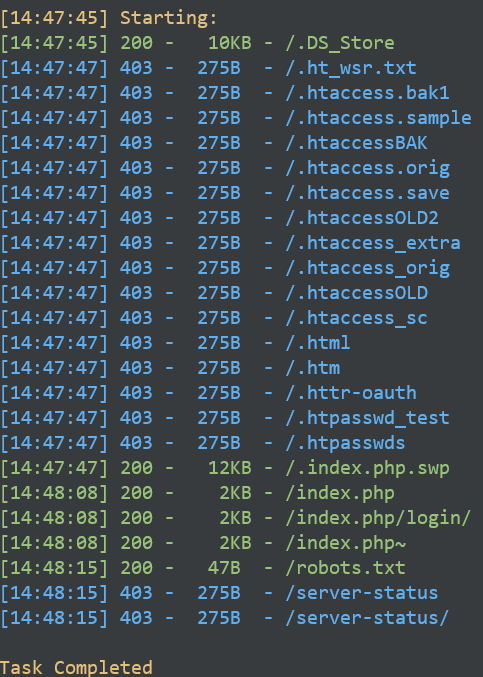
\includegraphics[width=0.5\textwidth]{1-web_junior/pic/1.jpg}
    \caption{扫描结果}
    \label{fig:pic1}
\end{figure}
那么把这些目录全部访问一遍。
\begin{itemize}
    \item 直接访问robots.txt: 提示flag在另一个文件中,再次访问得$ flag1:n1book\{info\_1 $
    \item 直接访问index.php$\sim$: $ flag2:s\_v3ry\_im $
    \item 恢复.index.php.swp: $ flag3:p0rtant\_hack\} $
\end{itemize}
拼凑起来,最终flag为:
\begin{lstlisting}
    n1book{info_1s_v3ry_imp0rtant_hack}
\end{lstlisting}

\newpage

\subsection{粗心的小李}
网页提示是很简单的git泄露,那么直接用\href{https://github.com/denny0223/scrabble}{scrabble}尝试恢复一下:
\begin{lstlisting}
    ./scrabble http://172.17.0.1
    重新初始化已存在的 Git 仓库于 /home/shijy/ctf/tools/web/scrabble/.git/
    parseCommit 213b7e386e9b0b406d91fae58bf8be11a58c3f88
    downloadBlob 213b7e386e9b0b406d91fae58bf8be11a58c3f88
    parseTree f46fbac4149604ca13a765950f9a2d1fd8c1c7ad
    downloadBlob f46fbac4149604ca13a765950f9a2d1fd8c1c7ad
    downloadBlob 1e0db5d96b5cc9785055c14bbec0e7ad14f48151
    HEAD 现在位于 213b7e3 flag
\end{lstlisting}

恢复成功,获得一个index.html文件,直接打开,搜索到flag:
\begin{lstlisting}
    n1book{git_looks_s0_easyfun}
\end{lstlisting}

\section{总结}
这两个问题都是有隐藏路径暴露在外网中,按道理上来直接目录扫描工具扫一下,之后再按情况分析即可。